\section{Simulation}

Die Grundlage der Simulation bildet die Grundschaltung und die Operationsverstärkerschaltung zur Aufbereitung des Shuntsignals $U_{R1}$ 
(Kapitel \ref{sec:Schaltung}). 
Die Schaltungen wurden in dem Simulationsprogramm LTspice\footnote{Wurde 1999 von Linear Technology einem 
US-Amerikanischen Halbleiter- und Softwarehersteller entwickelt.} aufgebaut. 
Zur Vereinfachung wurde $U_{U1+}$ mit einer Spannungsquelle simuliert und nicht mit der Schaltung $R2$ bis $R4$.
Die übrigen Widerstandswerte sind nach Tabelle \ref{tab:Werte_Fehler_Beispiel} festgelegt worden.
$Q1$ ist als ein IRFP240 \cite{IRFP250} simuliert.
Die Versorgungsspannungen und maximalen U/I-Werte der Last wurden nach Beispiel \ref{sec:Bsp} festgelegt.\\

\begin{table}[h!]
	\centering
	\caption{Beispiel Bauteile und Werte}
	\label{tab:Werte_Fehler_Beispiel}
	\normalsize
	\begin{tabular}{c|c|cc}
		Bauteil & Wert & Toleranz & $\Delta$ Wert\\
		\hline
		U2 bis U4 & LTC2057 & \cite{LTC2057} & --\\
		\multirow{2}{*}{R1}  & \multirow{2}{*}{\SI{100}{m\ohm}} & 0,5 \%,  & \multirow{2}{*}{0,762 m$\Omega$}\\
		&& TCR: 75 PPM/°C &\\
		R10 & $5 k\Omega$ & 1 \% & \SI{50}{\ohm} \\
		R11 & $15 k\Omega$ & 1 \%& \SI{150}{\ohm}\\
		R6  & $5 k\Omega$ & 1 \% & \SI{50}{\ohm} \\
		R7	& $5 k\Omega$ & 1 \% & \SI{50}{\ohm} \\
		R8  & $5 k\Omega$ & 1 \% & \SI{50}{\ohm} \\
		R9  & $20 k\Omega$ & 1 \%& \SI{200}{\ohm}\\
	\end{tabular}
\end{table}

\begin{figure}[!h]
	\centering
	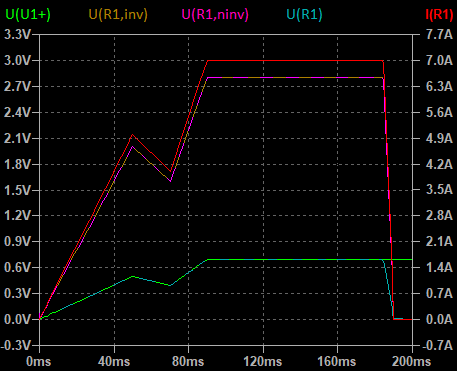
\includegraphics[width=0.45\textwidth]{Bilder/Simu_Kleinsignale.png}
	\renewcommand*\figurename{Diagramm}
	\caption{Simulation über 200ms für $U_{U1+}$, $U_{R1,inv}$, $U_{R1,ninv}$, $U_{R1}$ und $I_{R1}$}
	\label{simu:Kleinsignale}
\end{figure}

\begin{figure}[!h]
	\centering
	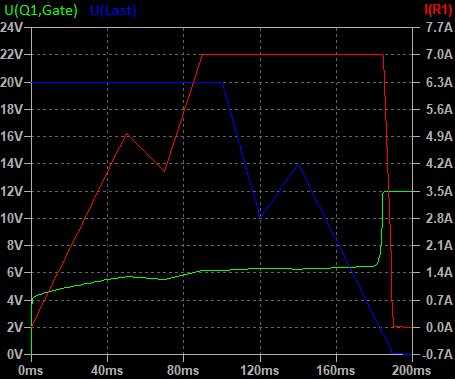
\includegraphics[width=0.45\textwidth]{Bilder/Simu_grossignale.png}
	\renewcommand*\figurename{Diagramm}
	\caption{Simulation über 200ms für $U_{Q1,Gate}$, $U_{Last}$ und $I_{R1}$}
	\label{simu:Großsignale}
\end{figure}


Im Diagramm \ref{simu:Kleinsignale} ist zu sehen, dass die Spannung $U_{U1+}$ bis \SI{90}{m\second} 
auf die festgelegten \SI{0,7}{\volt} eingestellt wird. Entsprechend folgt der gesteuerte Strom $I_{R1} = I_{Q1}$.
Die Spannung $U_{Q1,Gate}$ erhöht sich aufgrund der Gate-Source Schwellspannung nahezu sofort auf \SI{4}{\volt}.
Zu erkennen ist, dass bei einer Versorgungsspannung von \SI{5}{\volt} des Operationsverstärkers $U1$ der 
MOSFET $Q1$ für den gewünschten Strom von \SI{7}{\ampere} nicht genügend Gate-Source Spannung anlegen könnte.

Wenn ab $t \geq 100ms$ die Spannung an der Last linear sinkt, so ändert sich der Strom durch die Last nicht.
Ab einem $U_{Last} \lessapprox \SI{1,5}{\volt}$ ist der konstante Bereich erschöpft. 
An diesen Punkt kann der MOSFET $Q1$ keinen kleineren $R_{L}$ als $R_{L,min}$ (Formel \ref{eq:R_Lmin}) imitieren.
Für Spannungen $U_{Last} \lessapprox \SI{1,5}{\volt}$ gilt:

\begin{equation}
	I_{L} = \frac{U_{L}}{R_{L,min}}
\end{equation}

Ab einer Spannung $U_{Last} \lessapprox \SI{2}{\volt}$ steigt die Ausgangsspannung von $U1$ ($= U_{Q1,Gate}$) stark an, 
um $Q1$ niederohmiger zu schalten.
Diese Ausgangsspannung kann keinen Wert über \SI{12}{\volt} annehmen da dies das Maximum der Versorgung ist.

Die Schaltungen des invertierenden und nicht-invertierende Verstärkers verstärken beide, wie berechnet, 
die Shuntspannung $U_{R1}$ mit Faktor vier.


